\chapter{Rate Limiter}\label{ch:rate-limiter}

\resilienceMechanismChapterIntro{Rate Limiter}{proactive}


\section{Introduction}\label{sec:rate-limiter-introduction}

The Rate Limiter is a proactive resilience mechanism
that aims to control the rate at which requests are made to a service or resource.
By imposing a limit on the number of requests within a given time period,
the Rate Limiter helps to prevent overloading downstream services,
ensuring stability and availability~\cite{microsoft-rate-limiting-pattern,cloudflare-rate-limiting}.

Advantages of using a Rate Limiter include~\cite{solo-io-rate-limiting}:

\begin{itemize}
    \item \textbf{Prevent DoS Attacks and Web Scraping}:
    Rate limiting can help protect against denial-of-service (DoS) and distributed denial-of-service (DDoS) attacks and web scraping, making it harder for attackers to overwhelm a service with a high volume of requests.
    \item \textbf{Manage Resource Utilization}: By controlling the rate of requests, rate limiting helps to manage resource utilization, prevent resource starvation, and ensure that resources are available to all users.
    \item \textbf{Prevent Abuse}: Stops users from monopolizing resources and prevents excessive or unnecessary requests, ensuring fair resource distribution and optimal network or server performance.
    \item \textbf{Improve User Experience}: By controlling request rates,
    rate limiting reduces delays and enhances the responsiveness of the service for legitimate users, improving the overall user experience.
    \item \textbf{Reduce Costs}: It helps avoid extra costs associated with overloading resources, as limiting request rates reduces the demand on resources and prevents the need for additional capacity.
\end{itemize}

\subsection{API Gateway}\label{subsec:rate-limiter-api-gateway}

An API Gateway is a server or software application that acts as an intermediary between clients and backend services or microservices.
It serves as a single entry point for API calls, managing and routing them to the appropriate services, while also providing various functionalities to enhance security, performance, and usability.

One of the key features~\cite{api-gateway} of an API Gateway's traffic management is the implementation of rate limiting and throttling policies.
These policies control the rate of incoming requests and set rules and limits to regulate traffic, preventing the overloading of backend services.

\subsection{Relation To The Throttling Mechanism}\label{subsec:rate-limiter-throttling}

Rate limiting and throttling are closely related concepts often used interchangeably,
since both mechanisms control the rate of incoming requests to protect services from being overwhelmed, but they have distinct differences.
Rate limiting refers to the process of restricting the number of requests that can be made to a service within a given time period.
Throttling, on the other hand,
specifically adjusts the flow rate based on current system load.
Is typically used to ensure that high-priority requests are served first by delaying less critical ones.

To better illustrate the difference between these two concepts, consider the following analogy:
a rate limiter is like traffic lights that control the number of cars that can pass through an intersection within a certain time frame,
whereas throttling is like an adjustable hose nozzle that can be adjusted to control the flow of water, allowing more or less water to pass through based on the current water pressure.

\subsection{Semaphore}\label{subsec:rate-limiter-semaphore}

A semaphore is a synchronization primitive that restricts the number of simultaneous accesses to a shared resource up to a specified limit.
Key characteristics and operations of a semaphore include~\cite{java-semaphore, oracle-multithreaded-programming-guide}:

\begin{itemize}
    \item \textbf{Permits}: The semaphore keeps track of available permits.
    Each permit represents a single unit of resource access that can be granted.
    Resource access may require multiple permits, depending on the use case;
    \item \textbf{Acquire}: This operation decreases the number of available permits by a given number.
    If no permits are available, the acquiring entity is blocked (in the case of threads) or suspended (in the case of coroutines) until a permit is released;
    \item \textbf{Release}: This operation increases the number of available permits by a given number.
    Since releasing permits possibly created conditions for other entities (waiting to acquire permits) to proceed, then the semaphore notifies them.
\end{itemize}

There are two main types of semaphores:
\begin{itemize}
    \item \textbf{Binary Semaphore}:
    This type has only two states: available (1 permit) and unavailable (0 permits).
    In literature, it is also misconceptionally known as a mutex (mutual exclusion lock), but differs in ownership.
    An acquired mutex can only be released by the entity that acquired it, while a semaphore can be signalled by any other entity.
    \item \textbf{Counting Semaphore}: This type can have a count greater than one, allowing multiple entities to acquire permits up to a specified limit.
    It is used for managing access to a resource pool.
\end{itemize}

In the context of rate limiting, a semaphore can be used to control the rate of incoming requests by granting or denying access based on the availability of permits.

\subsection{Rate Limiting Algorithms}\label{subsec:rate-limiter-algorithms}

There are several algorithms that can be used to implement rate limiting,
each with its own characteristics and trade-offs~\cite{medium-rate-limiting-algorithms,nordic-apis-rate-limiting-algorithms}:

\subsubsection{Token Bucket}\label{subsubsec:token-bucket-algorithm}

This algorithm is used in packet-switched and telecommunications networks
to check data transmissions against defined limits on bandwidth and burstiness
(a measure of unevenness or variations in traffic flow).
The token bucket algorithm is based on the concept of a bucket that holds tokens,
where each token represents a unit of data or a permit to transmit data.
The key features of the token bucket algorithm include:

\begin{itemize}
    \item Has a fixed capacity (maximum number of tokens it can hold) and a refill rate (tokens added per unit of time);
    \item Tokens are added to the bucket at a constant rate, up to the maximum capacity;
    \item When a packet arrives, it must acquire a token from the bucket to proceed;
    \item If no tokens are available, the packet is considered non-conformant and may be dropped or delayed.
\end{itemize}

Provides a variable request rate and is suitable for handling bursts of requests,
as long as the bucket has enough tokens to accommodate them.
This algorithm can be implemented by a semaphore with no release operation, as the permits are automatically refilled at a constant rate.

\subsubsection{Leaky Bucket}\label{subsubsec:leaky-bucket-algorithm}

It is analogous to a bucket with a hole in the bottom that leaks water at a constant rate.
When water is poured into the bucket, it accumulates up to a certain level before overflowing.
Independent of the rate at which data is received,
the leaky bucket algorithm regulates the rate at which data is sent out by leaking it at a constant rate.
This way maintaining a constant output rate and preventing congestion.

In contrast to the token bucket algorithm,
the leaky bucket algorithm does not allow bursts of traffic to be accommodated.
Instead, it enforces a constant output rate by discarding excess data, which can be a disadvantage in some scenarios.

\subsubsection{Fixed Window Counter}\label{subsubsec:fixed-window-counter-algorithm}

The fixed window counter algorithm is an algorithm
that counts the number of requests made within discrete, fixed time intervals.

The key features of the fixed window counter algorithm include:

\begin{itemize}
    \item Requests are counted within a fixed time window (e.g., 1 second, 1 minute);
    \item When a request is made, the counter is incremented;
    \item If the counter exceeds the rate limit, the request is rejected;
    \item The counter is resetted at the beginning of each time window.
\end{itemize}

The fixed window counter algorithm is easy to implement but can lead to bursty traffic patterns,
as requests are not evenly distributed within the time window.
For example, if the rate limit is 5 requests per minute and a user made 5 requests at the end of the time window,
they circumvent the rate limit by making 5 more requests at the beginning of the next time window,
as demonstrated in Figure~\ref{fig:fixed-window-counter-problem}.
Essentially, violating the rate limit policy by doubling the number of allowed requests.

\begin{figure}[!htb]
    \centering
    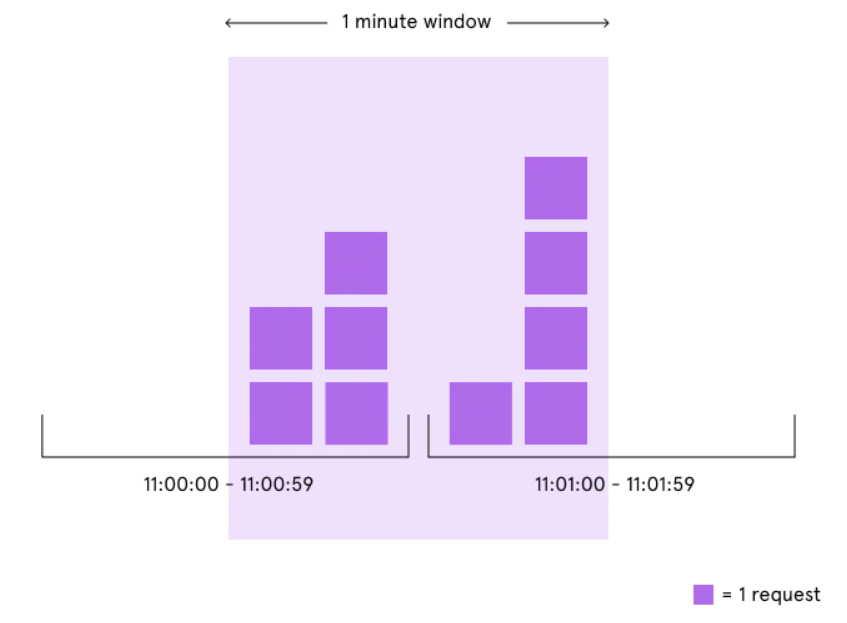
\includegraphics[width=0.5\textwidth]{../figures/06_fixed-window-counter-problem}
    \caption{Fixed Window Counter Problem.
    Retrieved from~\cite{medium-rate-limiting-algorithms}}.
    \label{fig:fixed-window-counter-problem}
\end{figure}

\subsubsection{Sliding Window Log}\label{subsubsec:sliding-window-log-algorithm}

In contrast to the fixed window counter algorithm, the sliding window log algorithm does not limit the requests based on a fixed time unit.
Instead, it maintains a continuous record of requests over a rolling time period.

The key features of the sliding window log algorithm include:

\begin{itemize}
    \item Tracks requests using a continuously moving window (e.g., last 60 seconds);
    \item Maintains a log of timestamps for each request within the sliding window;
    \item When a request is made, it checks the log to determine the number of requests within the current window;
    \item If the number of requests within the sliding window exceeds the rate limit, the request is rejected;
    \item The sliding window continuously updates, ensuring smooth rate limiting by taking the previous time interval into account.
\end{itemize}

The sliding window log algorithm smooths out traffic by avoiding the burstiness issue of fixed windows.
This is achieved by dynamically adjusting to the actual timing of requests, providing a more even distribution of allowed requests over time.
However, this algorithm continues to count requests even after the client exceeds the rate limit, which could leave a considerably large memory footprint because it stores a value for every request.

\subsubsection{Sliding Window Counter}\label{subsubsec:sliding-window-counter-algorithm}

Similar to the sliding window log algorithm, the sliding window counter algorithm aims to provide smooth rate limiting over a rolling time period.
However, it differs in implementation by maintaining a count of requests within fixed segments of the sliding window, rather than storing individual request timestamps.

The key features of the sliding window counter algorithm include:

\begin{itemize}
    \item Divides the time window into smaller fixed segments (e.g., 1-second segments within a 60-second window);
    \item Maintains a count of requests for each segment;
    \item When a request is made, it calculates the total number of requests in the current window by summing the counts of the relevant segments;
    \item If the total number of requests within the sliding window exceeds the rate limit, the request is rejected;
    \item The sliding window updates by shifting the segments as time progresses, ensuring that the count remains accurate for the current window.
\end{itemize}

The sliding window counter algorithm offers a more efficient implementation compared to the sliding window log, as it reduces the overhead of maintaining a detailed log of individual request timestamps.

\subsection{Rate Limit Exceeded}\label{subsec:rate-limiter-exceeded}

Rate limiting algorithms can deploy different strategies for handling requests when the rate limit is exceeded.
There are several strategies that can be used to manage requests when the rate limit is exceeded, including:

\begin{itemize}
    \item \textbf{Reject}: Immediately deny the request and return an error response message (e.g., throwing an exception,
    returning an HTTP status code such as 429 - Too Many Requests), indicating that the rate limit has been reached;
    \item \textbf{Wait}: Place the request in a queue to be processed later when the rate limit allows, ensuring that the request is not lost and will eventually be handled;
    \item \textbf{Both}: Combine the previous two approaches by placing the request in a queue with a timeout.
    If the request cannot be processed within the timeout period, it is rejected.
\end{itemize}


\section{Configuration}\label{sec:rate-limiter-configuration}

TODO()

\section{Implementation Aspects}\label{sec:rate-limiter-implementation}

TODO(revisit)

\subsection{Available Solutions}\label{subsec:rate-limiter-solutions}

TODO()

\subsection{Distribution}\label{subsec:rate-limiter-distribution}

TODO()


\subsection{Components}\label{subsec:rate-limiter-components}

\begin{itemize}
    \item \textbf{Semaphore}: To manage the acquisition and release of permits for requests in a synchronized way.
    This is used to control access to the shared resources (e.g., the rate-limited service) and is conceptually similar to the token bucket algorithm, where a token represents a permit;
    \item \textbf{Queue}: To hold requests when the rate limit is exceeded;
    \item \textbf{Shared Store}: The \texttt{Queue} and \texttt{Semaphore} components require shared state management (e.g., a database) to ensure consistency across multiple, possibly load-balanced, server instances.
\end{itemize}

